%%%%%%%%%%%%%%%%%%%%%%%%%%%%%%%%%%%%%%%%%
% a0poster Landscape Poster
% LaTeX Template
% Version 1.0 (22/06/13)
%
% The a0poster class was created by:
% Gerlinde Kettl and Matthias Weiser (tex@kettl.de)
% 
% This template has been downloaded from:
% http://www.LaTeXTemplates.com
%
% License:
% CC BY-NC-SA 3.0 (http://creativecommons.org/licenses/by-nc-sa/3.0/)
%
%%%%%%%%%%%%%%%%%%%%%%%%%%%%%%%%%%%%%%%%%

%----------------------------------------------------------------------------------------
%	PACKAGES AND OTHER DOCUMENT CONFIGURATIONS
%----------------------------------------------------------------------------------------

\documentclass[a0,landscape]{a0poster}

\usepackage{multicol} % This is so we can have multiple columns of text side-by-side
\columnsep=100pt % This is the amount of white space between the columns in the poster
\columnseprule=3pt % This is the thickness of the black line between the columns in the poster

\usepackage[svgnames]{xcolor} % Specify colors by their 'svgnames', for a full list of all colors available see here: http://www.latextemplates.com/svgnames-colors

\usepackage{times} % Use the times font
%\usepackage{palatino} % Uncomment to use the Palatino font
\usepackage{float} % Allows putting an [H] in \begin{figure} to specify the exact location of the figure
\usepackage{graphicx} % Required for including images
\graphicspath{{figures/}} % Location of the graphics files
\usepackage{booktabs} % Top and bottom rules for table
\usepackage[font=small,labelfont=bf]{caption} % Required for specifying captions to tables and figures
\usepackage{amsfonts, amsmath, amsthm, amssymb} % For math fonts, symbols and environments
\usepackage{wrapfig} % Allows wrapping text around tables and figures
\usepackage[center]{titlesec}
\usepackage{euler}
\begin{document}

%----------------------------------------------------------------------------------------
%	POSTER HEADER 
%----------------------------------------------------------------------------------------

% The header is divided into three boxes:
% The first is 55% wide and houses the title, subtitle, names and university/organization
% The second is 25% wide and houses contact information
% The third is 19% wide and houses a logo for your university/organization or a photo of you
% The widths of these boxes can be easily edited to accommodate your content as you see fit

\begin{minipage}[b]{0.55\linewidth}
\veryHuge \color{NavyBlue} \textbf{Radio Cosmology Lab} \color{Black}\\ % Title
\Huge\textit{Exploring the Epoch of Reionization}\\[1cm] % Subtitle
\huge \textbf{Joshua Kerrigan, Adam Lanman, Wenyang Li}\\ % Author(s)
\huge Brown University Physics\\ % University/organization
\end{minipage}
%
\begin{minipage}[b]{0.25\linewidth}
\color{DarkSlateGray}\Large \textbf{Contact Information:}\\
Physics\\ % Address
Brown University\\
$\#$ George St., Providence, RI\\\\
Phone: +1 (000) 111 1111\\ % Phone number
Email: \texttt{Add Emails}\\ % Email address
\end{minipage}
%
\begin{minipage}[b]{0.19\linewidth}

\includegraphics[width=20cm]{brown-logo.png} % Logo or a photo of you, adjust its dimensions here
\end{minipage}

\vspace{1cm} % A bit of extra whitespace between the header and poster content

%----------------------------------------------------------------------------------------

\begin{multicols}{4} % This is how many columns your poster will be broken into, a poster with many figures may benefit from less columns whereas a text-heavy poster benefits from more

%----------------------------------------------------------------------------------------
%	ABSTRACT
%----------------------------------------------------------------------------------------

\color{Navy} % Navy color for the abstract

\begin{abstract}

Following the recombination of hydrogen and release of the cosmic microwave background radiation at redshift $z \sim 1100$, the baryonic matter of the universe consisted mostly of neutral hydrogen and helium. Gradually, small inhomogeneities collapsed and ignited the first luminous structures. Energetic photons emitted from the first stars and quasars reionized the surrounding medium, producing ionized bubbles which grew and merged into the fully ionized intergalactic medium we see today. This \emph{Epoch of Reionization} (EoR) remains a poorly-understood period of the universe's history which offers a wealth of cosmological and astrophysical information.

The Pober lab is part of an international effort to build instruments capable of studying the EoR. The neutral hydrogen (HI) of the EoR emits faintly at a wavelength of 21cm, due to the hyperfine transition. This emission is unique to neutral hydrogen, and is anti-correlated with the ionized (HII) regions that fill the universe through the EoR. CMB constraints and quasar absorption spectra put the EoR as occurring within the redshift range $6 < z < 12$, which means 21cm emissions will redshift to meter scale wavelengths. This is accessible to modern radio interferometers, including the \emph{Donald C. Backer Precision Array for Probing the Epoch of Reionization} (PAPER), the \emph{Murchison Widefield Array} (MWA), and the recently-funded \emph{Hydrogen Epoch of Reionization Array} (HERA).

%The main focus of the Pober Lab is the direct observation of the 21cm Neutral Hydrogen (HI) emission through the use of radio telescope arrays to detect the signal from the Epoch of Reionization (EoR). The 21cm hyperfine spin flip, which is typically a forbidden transition, has a mean lifetime on the order of 100 million years. This time scale, and the abundance of HI in the universe gives us the ability to map the progress of reionization which has the redshift range of 6 $<$ z $<$ 12. To observe the reionization of the HI, we use radio telescope arrays, because the 21cm emission corresponds to 1420 MHz at rest and when received at Earth corresponds to 100-200 MHz due to cosmological redshifting. The Pober Lab contributes to several international radio telescope array collaborations which include the Precision Array for Probing the Epoch of Reionization (PAPER), the Murchison Widefield Array (MWA) and the newly NSF funded Hydrogen Epoch of Reionization Array (HERA).

\end{abstract}

%----------------------------------------------------------------------------------------
%	INTRODUCTION
%----------------------------------------------------------------------------------------

\color{SaddleBrown} % SaddleBrown color for the introduction

\section*{Introduction}

[The spin-flip transition and global history of the signal. Good place for pictures of bubble simulations]



\begin{figure}[H]
\centering
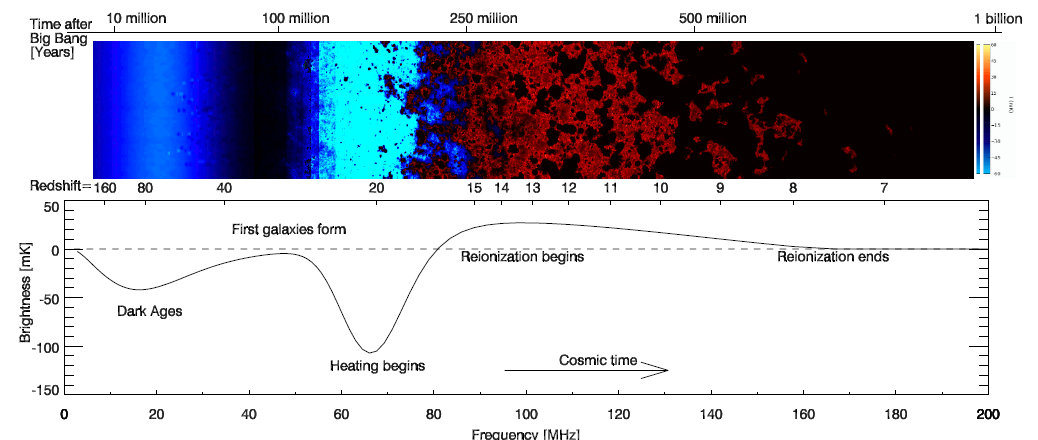
\includegraphics[width=1.0\linewidth]{figures/global_history.png}
\caption{The global differential brightness temperature, $\delta T_b$, evolution over redshift 6 $<$ z $<$ 160. $\delta T_b$ becomes observable when 
the spin temperature $T_S$ decouples from the CMB temperature, $T_{CMB}$ through the Wouthyusen-Field effect, this can be seen in 
Eqn. \ref{difftemp}}.
\end{figure}


\subsubsection*{Differential Brightness Temperature}
\begin{equation}
\label{difftemp}
\resizebox{.9\hsize}{!}{$
\delta T_{b} = 28mK(1+\delta)x_{HI}\Big(1-\frac{T_{CMB}}{T_{spin}}\Big)\Big(\frac{\sigma_{b}h^2}{0.0223}\Big)\sqrt{\Big(\frac{1+z}{10}\Big)\Big(\frac{0.24}{\sigma_m}\Big)}\Big[ \frac{H(z)/(1+z)}{dv_{||}/dr_{||}}\Big]$}
\end{equation}
The differential brightness temperature describes the complex nature of the neutral hydrogen spin temperature,$T_S$ decoupling from the CMB background temperature $T_{CMB}$, the neutral fraction of Hydrogen, $x_{HI}$, and the mass density contrast, $\delta$.
$\delta T_b$ also describes an important relationship between cosmological and astrophysical parameters, showing that measuring what is seen as a cosmological epoch has astrophysical relevance. 


%----------------------------------------------------------------------------------------
%	OBJECTIVES
%----------------------------------------------------------------------------------------
\color{DarkSlateGray} % DarkSlateGray color for the rest of the content
\subsection*{The Foreground Problem}
Galactic and extragalactic foregrounds pose a difficult problem when trying to measure the 21cm EoR signal. Relative to galactic foregrounds, the EoR signal is $\sim$ 5 orders of magnitude smaller than the galactic emissions that exist between our observing radio telescope arrays and the highly redshifted 21cm signal. The overlapping sources of power in our observations can be seen in Fig. \ref{foregroundsrcs}.


\begin{figure}[H]
\centering
\label{foregroundsrcs}
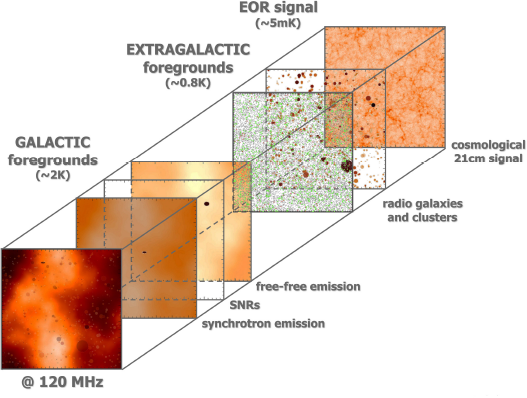
\includegraphics[width=0.55\linewidth]{figures/foreground_figure.png}
\caption{The various cosmological and galactic sources that contribute to the measured sky temperature, and their relative strengths. Source: Saleem Zaroubi, https://ned.ipac.caltech.edu/level5/March14/Zaroubi/Zaroubi5.html}
\end{figure}

The issue of foreground emission dominance in our power spectrum can be overcome through the mixed use of the following traditional and novel foreground mitigation techniques. \\
\subsubsection*{Foreground Subtraction}
\subsubsection*{Foreground Avoidance}
\subsubsection*{Inverse Covariance Weighting}




%----------------------------------------------------------------------------------------
%	MATERIALS AND METHODS
%----------------------------------------------------------------------------------------

\section*{Simulation}

[Diagram of the analysis pipeline, and power spectra from simulations. Emphasize the necessity of end to end simulation]

Fusce magna risus, molestie ut porttitor in, consectetur sed mi. Vestibulum ante ipsum primis in faucibus orci luctus et ultrices posuere cubilia Curae; Pellentesque consectetur blandit pellentesque. Sed odio justo, viverra nec porttitor vel, lacinia a nunc. Suspendisse pulvinar euismod arcu, sit amet accumsan enim fermentum quis. In id mauris ut dui feugiat egestas. Vestibulum ac turpis lacinia nisl commodo sagittis eget sit amet sapien. Phasellus imperdiet, tortor vitae congue bibendum, felis enim sagittis lorem, et volutpat ante orci sagittis mi. Morbi rutrum laoreet semper. Morbi accumsan enim nec tortor consectetur non commodo nisi sollicitudin. Proin sollicitudin. Pellentesque eget orci eros. Fusce ultricies, tellus et pellentesque fringilla, ante massa luctus libero, quis tristique purus urna nec nibh. Proin sollicitudin. Pellentesque eget orci eros. Fusce ultricies, tellus et pellentesque fringilla, ante massa luctus libero, quis tristique purus urna nec nibh.

%------------------------------------------------

\section*{Calibration}

[Calibration on sky sources and by redundancy. Wenyang's Figures of the calibrated visibilities would go well here.]

\begin{enumerate}
\item Lorem ipsum dolor sit amet, consectetur.
\item Nullam at mi nisl. Vestibulum est purus, ultricies cursus volutpat sit amet, vestibulum eu.
\item Praesent tortor libero, vulputate quis elementum a, iaculis.
\item Phasellus a quam mauris, non varius mauris. Fusce tristique, enim tempor varius porta, elit purus commodo velit, pretium mattis ligula nisl nec ante.
\item Ut adipiscing accumsan sapien, sit amet pretium.
\item Estibulum est purus, ultricies cursus volutpat
\item Nullam at mi nisl. Vestibulum est purus, ultricies cursus volutpat sit amet, vestibulum eu.
\item Praesent tortor libero, vulputate quis elementum a, iaculis.
\end{enumerate}

%----------------------------------------------------------------------------------------
%	RESULTS 
%----------------------------------------------------------------------------------------

\section*{Radio Telescope Arrays}

[Should probably move this section earlier. Description and pictures of the MWA Phase II, PAPER-64, and HERA-19. Good place to explain redundancy in the configurations]

Donec faucibus purus at tortor egestas eu fermentum dolor facilisis. Maecenas tempor dui eu neque fringilla rutrum. Mauris \emph{lobortis} nisl accumsan. Aenean vitae risus ante. Pellentesque condimentum dui. Etiam sagittis purus non tellus tempor volutpat. Donec et dui non massa tristique adipiscing.
%
\begin{wraptable}{l}{12cm} % Left or right alignment is specified in the first bracket, the width of the table is in the second
\begin{tabular}{l l l}
\toprule
\textbf{Treatments} & \textbf{Response 1} & \textbf{Response 2}\\
\midrule
Treatment 1 & 0.0003262 & 0.562 \\
Treatment 2 & 0.0015681 & 0.910 \\
Treatment 3 & 0.0009271 & 0.296 \\
\bottomrule
\end{tabular}
\captionof{table}{\color{Green} Table caption}
\end{wraptable}
%
Phasellus imperdiet, tortor vitae congue bibendum, felis enim sagittis lorem, et volutpat ante orci sagittis mi. Morbi rutrum laoreet semper. Morbi accumsan enim nec tortor consectetur non commodo nisi sollicitudin. Proin sollicitudin. Pellentesque eget orci eros. Fusce ultricies, tellus et pellentesque fringilla, ante massa luctus libero, quis tristique purus urna nec nibh.

Nulla ut porttitor enim. Suspendisse venenatis dui eget eros gravida tempor. Mauris feugiat elit et augue placerat ultrices. Morbi accumsan enim nec tortor consectetur non commodo. Pellentesque condimentum dui. Etiam sagittis purus non tellus tempor volutpat. Donec et dui non massa tristique adipiscing. Quisque vestibulum eros eu. Phasellus imperdiet, tortor vitae congue bibendum, felis enim sagittis lorem, et volutpat ante orci sagittis mi. Morbi rutrum laoreet semper. Morbi accumsan enim nec tortor consectetur non commodo nisi sollicitudin.

\begin{center}\vspace{1cm}

\includegraphics[width=0.8\linewidth]{placeholder}
\captionof{figure}{\color{Green} Figure caption}
\end{center}\vspace{1cm}

In hac habitasse platea dictumst. Etiam placerat, risus ac.

Adipiscing lectus in magna blandit:

\begin{center}\vspace{1cm}
\begin{tabular}{l l l l}
\toprule
\textbf{Treatments} & \textbf{Response 1} & \textbf{Response 2} \\
\midrule
Treatment 1 & 0.0003262 & 0.562 \\
Treatment 2 & 0.0015681 & 0.910 \\
Treatment 3 & 0.0009271 & 0.296 \\
\bottomrule
\end{tabular}
\captionof{table}{\color{Green} Table caption}
\end{center}\vspace{1cm}

Vivamus sed nibh ac metus tristique tristique a vitae ante. Sed lobortis mi ut arcu fringilla et adipiscing ligula rutrum. Aenean turpis velit, placerat eget tincidunt nec, ornare in nisl. In placerat.

\begin{center}\vspace{1cm}

\includegraphics[width=0.8\linewidth]{placeholder}
\captionof{figure}{\color{Green} Figure caption}
\end{center}\vspace{1cm}

%----------------------------------------------------------------------------------------
%	CONCLUSIONS
%----------------------------------------------------------------------------------------

\color{SaddleBrown} % SaddleBrown color for the conclusions to make them stand out

\section*{Conclusions}

[Do we have conclusions?]

\begin{itemize}
\item Pellentesque eget orci eros. Fusce ultricies, tellus et pellentesque fringilla, ante massa luctus libero, quis tristique purus urna nec nibh. Phasellus fermentum rutrum elementum. Nam quis justo lectus.
\item Vestibulum sem ante, hendrerit a gravida ac, blandit quis magna.
\item Donec sem metus, facilisis at condimentum eget, vehicula ut massa. Morbi consequat, diam sed convallis tincidunt, arcu nunc.
\item Nunc at convallis urna. isus ante. Pellentesque condimentum dui. Etiam sagittis purus non tellus tempor volutpat. Donec et dui non massa tristique adipiscing.
\end{itemize}

\color{DarkSlateGray} % Set the color back to DarkSlateGray for the rest of the content

%----------------------------------------------------------------------------------------
%	FORTHCOMING RESEARCH
%----------------------------------------------------------------------------------------

\section*{Forthcoming Research}

[Picture of HERA-331?]

Vivamus molestie, risus tempor vehicula mattis, libero arcu volutpat purus, sed blandit sem nibh eget turpis. Maecenas rutrum dui blandit lorem vulputate gravida. Praesent venenatis mi vel lorem tempor at varius diam sagittis. Nam eu leo id turpis interdum luctus a sed augue. Nam tellus.

 %----------------------------------------------------------------------------------------
%	REFERENCES
%----------------------------------------------------------------------------------------

\nocite{*} % Print all references regardless of whether they were cited in the poster or not
\bibliographystyle{plain} % Plain referencing style
\bibliography{sample} % Use the example bibliography file sample.bib

%----------------------------------------------------------------------------------------
%	ACKNOWLEDGEMENTS
%----------------------------------------------------------------------------------------

\section*{Acknowledgements}

Etiam fermentum, arcu ut gravida fringilla, dolor arcu laoreet justo, ut imperdiet urna arcu a arcu. Donec nec ante a dui tempus consectetur. Cras nisi turpis, dapibus sit amet mattis sed, laoreet.

%----------------------------------------------------------------------------------------

\end{multicols}
\end{document}